The bar pointer model\index{Bar pointer model} (or dynamic bar pointer model), referred to as \bpmodel\ in this chapter, is a generative model that has been successfully applied for meter analysis tasks. The model assumes a hypothetical time pointer within a bar that progresses at the speed of the tempo to traverse through the bar and then reinitializes at the end of the bar to track the next bar. The model also assumes that specific bar length rhythm patterns\index{Rhythm pattern} are played in a bar depending on the rhythmic style, and uses these patterns to track the progression through the bar. These rhythmic patterns can be fixed \textit{a priori} or learned from data to build an observation model for each position in the bar. When learned from data, the rhythmic patterns are built using a signal representation derived from audio, most often from frame level audio features to preserve the temporal information in features. Progressing through the bar, the model can hence be used to sample the observation model and generate a rhythmic pattern that is possible and allowed in the rhythm style. The model allows for different metrical structures, tempi ranges and rhythm styles, providing a flexible framework for meter analysis. Though applied only for meter analysis from audio recordings in this dissertation, the \bpmodel\ can be applied even to symbolic music~\cite{whiteley:06:ismir}. \bpmodel\ can be represented as a \gls{DBN} with specific conditional dependence relations between the variables that lead to several variants and extensions of the model. The structure of the \bpmodel\ is shown in \figref{fig:dbn:bpm}.

In a \gls{DBN}, an observed sequence of features derived from an audio signal $\obsVar_{1:\nframes} = \{\obsVar_1, \ldots, \obsVar_\nframes\}$ is generated by a sequence of hidden (latent) variables $\hidVar_{1:\nframes} \!=\! \{\hidVar_1, \ldots, \hidVar_\nframes\}$, where $\nframes$ is the length of the feature sequence (number of audio frames in an audio excerpt). The joint probability distribution of hidden and observed variables factorizes as, 
\begin{equation}
P(\obsVar_{1:\nframes},\hidVar_{0:\nframes}) = P(\hidVar_{0}) \cdot \overset{\nframes}{\underset{k=1}{\prod}}  P(\hidVar_{k} \mid \hidVar_{k-1})\,P(\obsVar_{k} \mid \hidVar_{k}) \label{eqn:dbn:basic}
\end{equation}
where, $P(\hidVar_{0})$ is the initial state distribution, $P(\hidVar_{k} | \hidVar_{k-1})$ is the transition model, and $P(\obsVar_{k} | \hidVar_{k})$ is the observation model.
%
\subsubsection{Hidden variables}
\begin{figure}[t]
\centering
	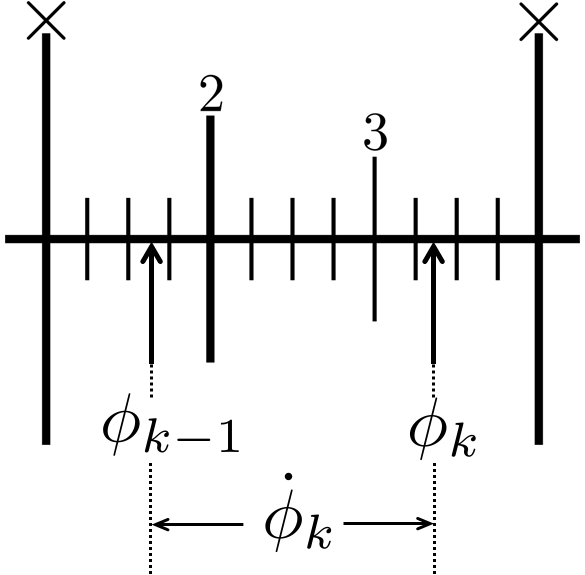
\includegraphics[scale=0.25]{meterTrack/bpm-illustration.pdf}
	\caption[An illustration of the bar pointer model]{An illustration of the progression of bar position and instantaneous tempo variables over two consecutive audio frames in a cycle of \gls{rupaka} \gls{tala}. The effect of instantaneous tempo is greatly exaggerated for clarity in the illustration.}
	\label{fig:bpm:illustration}
\end{figure}
%
In the bar pointer model, at each audio frame $k$, the hidden variable vector $\hidVar_{k}$ describes the state of a hypothetical bar pointer $\hidVar_{k} = [\mpos_k \; \tempoVar_k \; \rpattVar_k]$, representing the bar position, instantaneous tempo and a rhythmic pattern indicator, respectively (see \figref{fig:bpm:illustration} for an illustration).
%
\begin{itemize}[leftmargin=*]
\item \textit{Rhythmic pattern indicator}: The rhythmic pattern variable $\rpattVar \in \lbrace 1, \ldots, \nrhythmPatts\rbrace$ is an indicator variable to select one of the $\nrhythmPatts$ observation models corresponding to each bar (cycle) length rhythmic pattern of a rhythm class. Each pattern $\rpattVar$ has an associated length of cycle $\npos_\rpattVar$ and number of beat (or \gls{matra}) pulses $\nbeats_\rpattVar$. In the scope of this dissertation, all rhythmic patterns are learned from training data and not fixed \textit{a priori}. We can infer the rhythm class or meter type (\gls{tala}) by allowing rhythmic patterns of different lengths from different rhythm classes to be present in the model, as used by \citeA{krebs:15:pf}. However, it is to be noted that for the problem of meter tracking, we assume that the cycle length is known and that all the $\nrhythmPatts$ rhythmic patterns belong to the same rhythm class (\gls{tala}), $\npos_\rpattVar = \npos$ and $\nbeats_\rpattVar = \nbeats$~$\forall \, \rpattVar$. 

\item \textit{Bar position}: The bar position $\mpos \in [0, \npos_\rpattVar)$ variable indicates a position in the bar at any audio frame and tracks the progression through the bar. Here, $\npos_\rpattVar$ is the length of the bar (cycle), which is also the length of the bar length rhythmic pattern being tracked. The bar position variable traverses the whole bar and wraps around to zero at the end of the bar to track the next bar. The maximum value of bar (cycle) length, $\npos$, depends on the longest bar (cycle) that is tracked. We set the length of the longest bar being tracked to a fixed value, and scale other bar (cycle) lengths accordingly. 
\item \textit{Instantaneous tempo}: Instantaneous tempo $\tempoVar$ is the rate at which the bar position variable progresses through the cycle at each time frame, measured in bar positions per time frame. The range of the variable $\tempoVar_k \in [\tempoVar_{\min}, \tempoVar_{\max}]$ depends on the length of the cycle $\npos$ and the analysis frame hop size ($\framehop = $ 0.02 second used in this thesis), and can be preset or learned from data. A tempo value of $\tempoVar_{k}$ corresponds to a bar (cycle) length of ($\framehop \cdot \npos_\rpattVar / \tempoVar_{k}$) seconds and ($60 \cdot \nicefrac{\nbeats\cdot\tempoVar_k}{(\npos \cdot\framehop)})$ beats/\glspl{matra} per minute. The range of the variable can be used to restrict the range of tempi that is allowed within each rhythm class. 
\end{itemize}
\subsubsection{Initial state distribution}
The initial state distribution $P(\hidVar_{0})$ can be used to incorporate prior information about the metrical structure of the music into the model. Different initializations are explored depending on the meter analysis task under consideration. A uniform initialization is used for meter inference and tracking, while a narrower informed initialization is done for informed meter tracking. 
\subsubsection{Transition model}
Given the conditional dependence relations between the variables of the \bpmodel\ in \figref{fig:dbn:bpm}, the transition model factorizes as, 
\begin{multline}\label{eqn:bpm:transx}
P(\hidVar_{k} \mid \hidVar_{k-1})=P(\mpos_{k} \mid \mpos_{k-1},\tempoVar_{k-1},\rpattVar_{k-1})P(\tempoVar_{k} \mid \tempoVar_{k-1}) \\ P(\rpattVar_{k} \mid \rpattVar_{k-1},\mpos_{k},\mpos_{k-1})
\end{multline}
The individual terms of the equation can be expanded as, 
\begin{equation}\label{eqn:bpm:transmpos}
P(\mpos_{k} \mid \mpos_{k-1},\tempoVar_{k-1},r_{k-1})=\indicator_{\mpos}
\end{equation}
where $\indicator_{\mpos}$ is an indicator function that takes a value of one if $\mpos_{k} = (\mpos_{k-1} + \tempoVar_{k-1})\!\!\!\mod\!\!(\npos_{\rpattVar_{k-1}})$ and zero otherwise. The tempo transition is given by,
\begin{equation}\label{eqn:bpm:transtempo}
P(\tempoVar_{k} \mid \tempoVar_{k-1})\propto\mathcal{N}(\tempoVar_{k-1},\sigma_{\tempoVar_k}^{2})\times \indicator_{\tempoVar}
\end{equation}
where $\indicator_{\tempoVar}$ is an indicator function that equals one if $\tempoVar_{k} \in [\tempoVar_{\textrm{min}}, \tempoVar_{\textrm{max}}]$ and zero otherwise, restricting the tempo to be between a predefined range. $\normDist(\mu,\sigma^2)$ denotes a normal distribution with mean $\mu$ and variance $\sigma^{2}$. The value of $\sigma_{\tempoVar_{k}}$ depends on the value of tempo to allow for larger tempo variations at higher tempi. % and the length of the pattern, \cdot (\nicefrac{\npos_{\rpattVar_{k-1}}}{\npos})
We set $\sigma_{\tempoVar_k} = \sigma_n \cdot \tempoVar_{k-1}$, where $\sigma_n$ is a user parameter that controls the amount of local tempo variations we allow in the music piece. The pattern transitions are governed by, 
\begin{equation}\label{eqn:bpm:transpatt}
P(\rpattVar_{k} \mid \rpattVar_{k-1},\mpos_{k},\mpos_{k-1}) = 
\begin{cases}
 \tmPatt(\rpattVar_{k-1},\rpattVar_{k}) & \text{if} \,\,\, \mpos_{k} < \mpos_{k-1}\\
\indicator_{\rpattVar} & \text{else}
\end{cases}
\end{equation}
where, $\tmPatt$ is the $\nrhythmPatts \times \nrhythmPatts$ time-homogeneous transition matrix with $\tmPatt(i, j)$ being the transition probability from $\rpattVar_i$ to $\rpattVar_j$, and $\indicator_{r}$ is an indicator function that equals one when $\rpattVar_k = \rpattVar_{k-1}$ and zero otherwise. Since the rhythmic patterns are one bar (cycle) in length, pattern transitions are allowed only at the end of the bar (cycle). When there are multiple patterns, these transition probabilities indicate the most probable movement through these patterns from bar to bar, as the piece progresses. To reflect the performance practice, the pattern transition probabilities are learned from data.
\subsubsection{Observation model}
The observation model aims to model the underlying rhythmic patterns present in the metrical structure being inferred/tracked, explaining the possible rhythmic events at each position in the bar. Some of the positions in a bar have a higher probability of an onset occurring than other parts (e.g. the positions corresponding to downbeats, beats). Further, the strength of these onsets also vary depending on accent patterns of a rhythm class (which can be modeled from labeled data). The observation model used in this dissertation aims to address both these aspects (the locations and strengths of the rhythmic events), and closely follows the observation model proposed by \citeA{krebs:13:bpm}. 

The utility of spectral flux based rhythmic audio features was outlined in preliminary experiments \secref{sec:mt:earlyexpts}. A similar audio derived spectral flux\index{Spectral flux} feature is used in this dissertation as well, identical to features used by \citeA{krebs:13:bpm}, as explained in \secref{sec:cmrdataset} (see \figref{fig:obs:featcomp}). Since the bass onsets have significant information about the rhythmic patterns, the features are computed in two frequency bands (Low: $\leq$ 250 Hz, High: $>$ 250 Hz). 

It is assumed that the audio features depend only on the bar position and rhythmic pattern variables, without any influence from tempo. While this assumption is not completely true, it simplifies the observation model and helps to train better models with limited training data. Further, it is assumed that the audio features do not vary too much over short changes in position in cycle (e.g. the spectral flux variations within a small fraction of an \gls{akshara} might be negligible), which additionally helps to tie several positions to have the same observation probability and helps train models with limited training data.

Using beat and downbeat annotated training data, the audio features are then grouped into bar length patterns. The bar is then discretized into 64$^{\mathrm{th}}$ note cells (four cells per \gls{akshara} for Carnatic music, and four cells per \gls{matra} for Hindustani music, corresponds to $25$ bar positions with $\npos = 1600$). A k-means clustering algorithm clusters and assigns each bar of the dataset to one of the $\nrhythmPatts$ rhythmic patterns. All the features within the cell are then collected for each pattern, and maximum likelihood estimates of the parameters of a two component \gls{GMM} are obtained. The observation probability within a 64$^{\mathrm{th}}$ note cell is assumed to be constant, and computed as, 
\begin{equation}\label{eqn:bpm:obsmodel}
P(\obsVar \mid \hidVar) = P(\obsVar \mid \mpos,\rpattVar) = \overset{2}{\underset{i=1}{\sum}}\pi_{\mpos,\rpattVar,i}\,\normDist(\obsVar;\boldsymbol{\mu}_{\mpos,\rpattVar,i},\boldsymbol{\Sigma}_{\mpos,\rpattVar,i})
\end{equation}
where, $\normDist(\obsVar;\boldsymbol{\mu},\boldsymbol{\Sigma})$ denotes a normal distribution of the two dimensional feature $\obsVar$. For the mixture component $i$, $\pi_{\mpos,\rpattVar,i}, \boldsymbol{\mu}_{\mpos,\rpattVar,i}$ and $\boldsymbol{\Sigma}_{\mpos,\rpattVar,i}$ are the component weight, mean (2-dimensional) and the covariance matrix ($2\times2$), respectively.
% 
\subsubsection{Inference in bar pointer model}
The goal of inference in meter analysis tasks is to find a hidden variable sequence that maximizes the posterior probability of the hidden states given an observed sequence of features: a \gls{MAP} sequence $\hidVar^{\optstar}_{1:\nframes}$ that maximizes $P(\hidVar_{1:\nframes} \mid \obsVar_{1:\nframes})$. The inferred hidden variable sequence $\hidVar^{\optstar}_{1:\nframes}$ can then be translated into a sequence of: 
\begin{itemize}[noitemsep]
	\item downbeat (\gls{sama}) instants: $\samaSet = \{\timeVar^{\optstar}_k \mid \mpos^{\optstar}_k = 0\}$
	\item beat instants: $\beatSet = \{\timeVar^{\optstar}_k \mid \mpos^{\optstar}_k = i \cdot \nicefrac{\npos_{\rpattVar^\optstar}}{\nbeats_{\rpattVar^\optstar}}$, $i = 1,\ldots,\nbeats_\rpattVar \}$
	\item local instantaneous tempo: $\tempoVar^{\optstar}_k$
	\item estimated rhythmic patterns: $\rpattVar^{\optstar}$
\end{itemize}
Two different inference schemes are now described, an inference using the Viterbi algorithm in a discretized state space, and an approximate inference using particle filters in the continuous space of $\mpos$ and $\tempoVar$, with the discrete variable $\rpattVar$. 
\subsubsection{Viterbi algorithm}
The continuous variables of bar position and tempo can be discretized, which transforms the \gls{DBN} into an \gls{HMM} over the cartesian product space of the discretized variables. In the \gls{HMM}, an inference can be performed using the Viterbi algorithm to compute the most likely sequence of hidden states given the observed feature sequence.  
% We follow the discretization that closely follows the method proposed by \citeA{krebs:15:pf}, by replacing the continuous variables $\mpos$ and $\tempoVar$ by their discretized counterparts, 
% \small
% \begin{eqnarray}
% 	m\!\!&\in&\!\!\{1,2,\ldots,\lceil \npos_\rpattVar \rceil\} \label{eqn:bpm:discmpos}\\
% 	n\!\!&\in&\!\!\{\tempoVar_{\min}, \tempoVar_{\min}\!+\!\deltatempo, \tempoVar_{\min}\!+\!2\deltatempo, \cdots, \tempoVar_{\max}\!-\!\deltatempo, \tempoVar_{\max}\} \label{eqn:bpm:disctempo}
% \end{eqnarray}
% \normalsize
% where $\deltatempo$ is the resolution of the tempo grid, and is computed as $\deltatempo = \nicefrac{(\tempoVar_{\max} - \tempoVar_{\min})}{(\ntempo-1)}$, where $\ntempo$ denotes the number of discrete tempo states. 
% 
% With such a discretization in place, the transition model equations \eqnref{eqn:bpm:transx}, \eqnref{eqn:bpm:transmpos} and \eqnref{eqn:bpm:transpatt} remain as defined. However, the tempo transition probability is redefined within the allowed tempo range as, 
% \begin{equation}
% P(n_{k} \mid n_{k-1}) = 
% \begin{cases}
% 1-p_{n} & \text{if} \,\,\, n_{k}=n_{k-1} \\
% \frac{p_n}{2} & \text{if} \,\,\, n_{k}=n_{k-1} \pm \deltatempo \\
% 0 & \text{otherwise}
% \end{cases}
% \end{equation}

We follow a discretization scheme that is identical to the method proposed by \citeA{krebs:15:pf}, by replacing the continuous variables $\mpos$ and $\tempoVar$ by their discretized counterparts $\mposDisc$ and $\tempoVarDisc$, respectively, as 
\begin{eqnarray}
	\mposDisc & \in & \{1,2,\ldots,\lceil \npos_\rpattVar \rceil\} \label{eqn:bpm:discmpos}\\
	\tempoVarDisc & \in & \{\tempoVarDisc_{\min}, \tempoVarDisc_{\min} + 1, \tempoVarDisc_{\min} + 2, \cdots, \ntempo - 1, \ntempo\} \label{eqn:bpm:disctempo}
\end{eqnarray}
Here, $\tempoVarDisc_{\min} = \lfloor \tempoVar_{\min} \rfloor$ and $\ntempo = \tempoVarDisc_{\max} = \lceil \tempoVar_{\max} \rceil$ is the discrete minimum and maximum tempo values allowed, where $\lfloor \cdot \rfloor$ and $\lceil \cdot \rceil$ denote floor and ceil operations, repsectively. 

With such a discretization in place, the transition model equations \eqnref{eqn:bpm:transx}, \eqnref{eqn:bpm:transmpos} and \eqnref{eqn:bpm:transpatt} remain as defined. However, the tempo transition probability is redefined within the allowed tempo range as, 
\begin{equation} \label{eqn:bpm:hmmntrans}
P(\tempoVarDisc_{k} \mid \tempoVarDisc_{k-1}) = 
\begin{cases}
1-p_{n} & \text{if} \,\,\, \tempoVarDisc_{k}=\tempoVarDisc_{k-1} \\
\frac{p_n}{2} & \text{if} \,\,\, \tempoVarDisc_{k}=\tempoVarDisc_{k-1} \pm 1 \\
0 & \text{otherwise}
\end{cases}
\end{equation}
where $p_n$ is the probability of tempo change. It is to be noted that that the discretization of $\mpos$ and $\tempoVar$ need not be done on an integer or on a uniform grid. It is possible that the tempo range can be non-uniformly sampled, as was proposed by \citeA{krebs:15:ismir}. In this dissertation, however, only a uniform discretization is explored in the context of the \gls{HMM}. Viterbi algorithm~\cite{rabiner:89:tutorial}\index{Viterbi decoding} is then used to obtain a \gls{MAP} sequence of states with the \gls{HMM}. The \gls{HMM} based Viterbi decoding inference algorithm in \bpmodel\ as described in the section will be denoted as \acrshort{hmmprior} in the dissertation. 

The drawback of this approach is that the discretization has to be on a very fine grid in order to guarantee good performance, which leads to a prohibitively large state space (specially with long cycles) and, as a consequence, to a computationally demanding inference. The size of the state space is $\mathfrak{S} = \npos \cdot \ntempo \cdot \nrhythmPatts$ and needs a $\mathfrak{S}\times\mathfrak{S}$ sized transition matrix. As an example, dividing a bar into $\npos = 1600$ position states, with $\ntempo = 15$ tempo states and $\nrhythmPatts = 4$ patterns, the size of the state space is $\mathfrak{S} = 96000$ states. The computational complexity of the Viterbi algorithm is $\bigO(\nframes\!\cdot\!\lvert \mathfrak{S} \rvert ^2)$. Even though the state transition matrix is sparse due to a lower number of allowed transitions leading to a complexity of $O(\nframes \cdot \npos \cdot \nrhythmPatts)$, the inference with \gls{HMM} can become computationally prohibitive and does not scale well with increasing number of states. This problem can be overcome, for instance, by using approximate inference methods such as particle filters. 
\subsubsection{Particle Filter (PF)}
Particle filters\index{Particle filter} (or \gls{SMC} methods) are a class of approximate inference algorithms to estimate the posterior density in a state space. They overcome two main problems of the \gls{HMM} - discretization of the state space and the quadratic scaling up of the size of state space with additional hidden variables. In addition, they can incorporate long term relationships between hidden variables. 

In the continuous state space of $\hidVar_{1:\nframes}$, the exact computation of the posterior $P(\hidVar_{1:\nframes}|\obsVar_{1:\nframes})$ is often intractable, but it can be evaluated pointwise. In particle filters, the posterior is approximated using a weighted set of points (known as particles) in the state space as,
\begin{equation}\label{eqn:bpm:pfposterior}
P(\hidVar_{1:\nframes} \mid \obsVar_{1:\nframes})\approx\overset{\nparticles}{\underset{i=1}{\sum}}w_{\nframes}^{(i)}\delta(\hidVar_{1:\nframes}-\hidVar_{1:\nframes}^{(i)})
\end{equation}
Here, $\{\hidVar^{(i)}_{1:\nframes}\}$ is a set of points (particles) with associated weights $\{\weight_{\nframes}^{(i)}\}$, $i = 1,\ldots,N_p$, $\hidVar_{1:\nframes}$ is the set of all state trajectories until frame $\nframes$, $\delta(x)$ is the Dirac delta function, and $\nparticles$ is the number of particles. 

With this particle system, starting with $P(\hidVar_0)$, to approximate the posterior pointwise, we need a suitable method to draw samples $\hidVar^{(i)}_k$ and compute appropriate weights $\weight_{k}^{(i)}$ recursively at each time step. It is clearly non-trivial to sample from an arbitrary posterior distribution. A simple approach is \gls{SIS}~\cite{doucet:09:tutorial}, where we sample from a \textsl{proposal} distribution $Q(\hidVar_{1:k} | \obsVar_{1:k})$ that has the same support and is as similar to the true (target) distribution $P(\hidVar_{1:k} | \obsVar_{1:k})$ as possible. To account for the fact that we sampled from a proposal and not the target, we attach an importance weight $\weight^{(i)}_k$ to each particle, computed as, 
\begin{equation}\label{eqn:bpminf:proposal}
\weight^{(i)}_{k} = \frac{P(\hidVar_{1:k} \mid \obsVar_{1:k})}{Q(\hidVar_{1:k} \mid \obsVar_{1:k})}
\end{equation}
With a suitable proposal density, these weights can be computed recursively as, 
\begin{equation}\label{eqn:bpminf:wtupdate}
\weight_{k}^{(i)}\propto \weight_{k-1}^{(i)}\frac{P(\obsVar_{k} \mid \hidVar_{k}^{(i)})P(\hidVar_{k}^{(i)} \mid \hidVar_{k-1}^{(i)})}{Q(\hidVar_{k}^{(i)} \mid \hidVar_{k-1}^{(i)},\obsVar_{k})}
\end{equation}
Following \citeA{krebs:15:pf}, we choose to sample from the transition probability $Q(\hidVar_{k}^{(i)} \mid \hidVar_{k-1}^{(i)},\obsVar_{k}) = P(\hidVar_{k}^{(i)} \mid \hidVar_{k-1}^{(i)})$, which reduces \eqnref{eqn:bpminf:wtupdate} to 
\begin{equation}\label{eqn:bpminf:wtSIS}
\weight_{k}^{(i)}\propto w_{k-1}^{(i)}P(\obsVar_{k} \mid \hidVar_{k}^{(i)})
\end{equation}
The \gls{SIS} algorithm derives samples by first sampling from proposal, in this case the transition probability and then computes weights according to \eqnref{eqn:bpminf:wtSIS}. Once we determine the particle trajectories $\{\hidVar^{(i)}_{1:\nframes}\}$, we then select the trajectory $\hidVar^{(i^{*})}_{1:\nframes}$ with the highest weight $\weight^{(i^{*})}_K$ as the \gls{MAP} state sequence. 

Many extensions have been proposed to the basic \gls{SIS} filter (\citeA{doucet:09:tutorial} provide a comprehensive overview) to address several problems with it. Some of the relevant extensions are briefly mentioned, emphasizing their key aspects. A more detailed description of the algorithms has been presented by \citeA{krebs:15:pf}. 

The most challenging problem in particle filtering is the degeneracy problem, where within a short time, most of the particles have a weight close to zero, representing unlikely regions of state space. This is contrary to the ideal case when we want the proposal to match well with the target distribution leading to a uniform weight distribution with low variance. To reduce the variance of the particle weights, resampling steps are necessary, which replace low weight particles with higher weight particles by selecting particles with a probability proportional to their weights. Several resampling methods have been proposed, but we use systematic resampling in this dissertation as recommended by \citeA{doucet:09:tutorial}. With resampling as the essential difference, the \gls{SIS} filter with resampling is called as \gls{SISR} filter. 

In meter analysis problems, due to metrical ambiguities, the posterior distribution $P(\hidVar_k | \obsVar_{1:k})$ is highly multimodal. Resampling tends to lead to a concentration of particles in one mode of the posterior, while the remaining modes are not covered. One way to alleviate this problem is to compress the weights $\weightVec_k = \{\weight^{(i)}_k\}$, $i = 1,\ldots, \nparticles$ by a monotonically increasing function to increase the weights of particles in low probability regions so that they can survive resampling. After resampling, the weights have to be uncompressed to give a valid probability distribution. This can be formulated as an \gls{APF} \cite{johansen:08:auxpf}.

A particle system that is capable of handling metrical ambiguities must maintain the multimodality of posterior distribution and be able to track several hypotheses together, which \gls{SISR} and \gls{APF} cannot do explicitly. A system called the \gls{MPF} was proposed by \citeA{vermaak:03:multimodal} to track multiple hypotheses, and was adapted to meter inference by \citeA{krebs:15:pf}. 

In a \gls{MPF}, each particle is assigned to a cluster that (ideally) represents a mode of the posterior. During resampling, the particles of a cluster interact only with particles of the same cluster. Resampling is done independently in each cluster, while maintaining the probability distribution intact. This way, all the modes of the posterior can be tracked through the whole audio piece, and the best hypothesis can be chosen at the end. In this work, we use an identical clustering scheme using a cyclic distance measure as described by \citeA{krebs:15:pf} to track several different possible metrical positions at a given time. We use a cyclic distance measure that can take into account the cyclic nature of the bar position $\mpos$. By representing the bar position as a complex phasor on the unit circle, we can compute the corresponding angle $\varphi(\mpos_k) = \nicefrac{2\pi \mpos_k}{\npos}$. A distance between two particles indexed by $i$ and $j$ can then be computed as, 
\begin{multline}
d(i,j)=\lambda_{\mpos}\left[\left(\cos(\varphi^{(i)})-\cos(\varphi^{(j)})\right)^{2}\!+\!\left(\sin(\varphi^{(i)})-\sin(\varphi^{(j)})\right)^{2}\right]\\
+\lambda_{\tempoVar}\left(\tempoVar^{(i)}-\tempoVar^{(j)}\right)^{2}+\lambda_{\rpattVar}(\rpattVar^{(i)}-\rpattVar^{(j)})^{2}
\end{multline}
where, the parameters $[\lambda_{\mpos}$, $\lambda_{\tempoVar}$, $\lambda_{\rpattVar}]$ control the relative weights in the distance. 

In the \gls{MPF}, after an initial cluster assignment, we perform a reclustering before every resampling step, merging or splitting clusters based on the average distance between cluster centroids. The clustering, merging and splitting of clusters is necessary to control the number of clusters, which ideally represents the number of modes in the posterior. The mixture particle filter can be combined with auxiliary resampling to give the \gls{AMPF}. As recommended by \citeA{krebs:15:pf}, we resample at a fixed interval $\sampInterval$. 
%
\begin{algorithm}
\caption{An outline of the \acrshort{pfprior} algorithm (\gls{AMPF} for inference in \bpmodel)}\label{algo:pf:prior}
  \begin{algorithmic}[1]
      \For{i = 1 to \nparticles} 
         \State Sample $\hidVar^{(i)}_0 \sim P(\hidVar_0)$  \Comment{$\hidVar_k = [\mpos_k,\tempoVar_k,\rpattVar_k]$}
         \State Set $\weight_{0}^{(i)} = \nicefrac{1}{\nparticles}$
      \EndFor
      \State Cluster $\{\hidVar^{(i)}_0 | i = 1, 2, \cdots, \nparticles\}$, get cluster assignments $\{\clust^{(i)}_0\}$
      % Main iteration
      \For{k = 1 to \nframes}
         \For{i = 1 to \nparticles} \Comment{\mpos, \rpattVar: Proposal and weights}
            \State Sample $\mpos^{(i)}_{k} \sim P(\mpos^{(i)}_{k} \mid \hidVar^{(i)}_{k-1})$, Set $\clust^{(i)}_k = \clust^{(i)}_{k-1}$
            \If{$\mpos^{(i)}_{k} < \mpos^{(i)}_{k-1}$}    \Comment{Bar crossed}
               \State $\rpattVar_k^{(i)} \sim P(\rpattVar_k^{(i)} \mid \rpattVar_{k-1}^{(i)})$ \Comment{Sample patterns}
            \Else
               \State $\rpattVar_k^{(i)} = \rpattVar_{k-1}^{(i)}$
            \EndIf
            \State $\tilde{\weight}_{k}^{(i)} = \weight_{k}^{(i)} \cdot P(\obsVar_{k} \mid \mpos_{k}^{(i)},\rpattVar_{k}^{(i)})$
         \EndFor
         % Normalize weights
         \For{i = 1 to \nparticles} \Comment{Normalize weights}
            \State $\weight_{k}^{(i)}=\frac{\tilde{\weight}_{k}^{(i)}}{\overset{\nparticles}{\underset{i=1}{\sum}}\tilde{\weight}_{k}^{(i)}}$
         \EndFor
         \If{$\mod(k,\sampInterval) = 0$}	\Comment{Cluster, resample, reassign}
            \State Cluster and resample $\{\hidVar_k^{(i)}, \weight_{k}^{(i)},\clust_k^{(i)} | i = 1, 2, \cdots, \nparticles\}$ \par
            \hskip\algorithmicindent \!\!to obtain $\{\hat\hidVar_k^{(i)}, \hat{\weight}_{k}^{(i)}\!=\!\nicefrac{1}{N_p},\hat{\clust}^{(i)}_{k}\}$
            \For{i = $1$ to $N_p$} 
               \State $\hidVar_k^{(i)} =  \hat{\hidVar}_k^{(i)}$, $\weight_k^{(i)} =  \hat{\weight}_k^{(i)}$, $\clust_k^{(i)} =  \hat{\clust}_k^{(i)}$
            \EndFor
         \EndIf
         \State Sample $\tempoVar^{(i)}_{k} \sim P(\tempoVar^{(i)}_{k} \mid \tempoVar^{(i)}_{k-1})$ \Comment{Sample tempo}
      \EndFor
      \State Compute $\hidVar^{\optstar}_{1:K} = \hidVar^{(i^{\optstar})}_{1:K} \mid i^{\optstar} = \argmax\limits_{i} {\weight^{(i)}_K}$ \Comment{\gls{MAP} sequence}% \argmax\limits_{i} will make i come below argmax
  \end{algorithmic}
\end{algorithm}

It has been clearly shown by \citeauthor{krebs:15:pf} that \gls{AMPF} can be effectively used for the task of meter inference and tracking. In this dissertation, the \gls{AMPF} algorithm, as outlined in \algoref{algo:pf:prior} is used for all meter analysis tasks that need approximate inference. The \gls{AMPF} algorithm with the \bpmodel\ as described in this section will be denoted as \acrshort{pfprior} in the dissertation. 

The complexity of the PF schemes scales linearly with the number of particles $\nparticles$ irrespective of the size of state space, leading to an efficient inference in large state spaces. Further, compared to the \gls{HMM} using Viterbi decoding that has a space complexity of $O(\nframes\!\cdot\!\lvert \mathfrak{S} \rvert)$, the PF needs to store just $\nparticles$ state trajectories and weights, significantly reducing the memory requirements. An additional advantage is that the number of particles can be chosen based on the computational power we can afford, and we can make the state space larger with no or only a marginal increase in the computational requirements. 

To conclude, the bar pointer model is a state of the art model useful in all the meter analysis that are addressed in the thesis. The performance of meter analysis with \bpmodel\ will be a baseline for all the datasets and music cultures under study. Though a state of the art model explored before, the dissertation presents a further exploration of the model with the following novelties compared to the previous approaches: 
\begin{enumerate}[leftmargin=*,noitemsep]
 \item The bar pointer model has been extended and evaluated on Indian art music, showing its utility and discussing its limitations with the kinds of metrical structures that occur in Indian music. These learnings and insights will help improve the components of the model, pushing the state of the art ahead. 
 \item Even though the bar pointer model can handle multiple rhythmic patterns per rhythm class (or meter type), only one previous study has applied it to include more than one rhythmic pattern per rhythm class~\cite{holzapfel:14:odd}. The dissertation for the first time applies the bar pointer model to multiple rhythm patterns per rhythm class and presents an evaluation. 
 \item Several novel extensions to the bar pointer model are explored and presented in the dissertation to address several shortcomings of the model, and to extend the functionality of the model. 
\end{enumerate}
%\note{What is the task of inference ? Formulate mathematically, and present formulation generic to HMM and PF inference schemes.}
%\comment{For each inference scheme, present an algorithm to explain how it works. Example if needed. }
% \subsubsection{HMM Viterbi inference}
% \note{HMM Viterbi inference: How we need to discretize the state space for that, what methods are available, and what are its implications. Present how the equations would change in this case.}
% \subsubsection{Particle Filter Inference}
% \note{Sequential Monte Carlo methods. Why they are good, what they are, basics referring to the background section.}
% \note{Inference in particle filters, SIS, SISR, APF, AMPF. Explain the algorithm in detail only for AMPF. }
%\comment{Algorithm listings for AMPF, AMPF\_mix, AMPF\_SPM, AMPF\_``full"}